\pdfminorversion=7
%%
%% ========== TITLE INFORMATION ==========
%%
%% Thesis type: DA ... diploma thesis, DISS ... PhD thesis
\newcommand{\thesistype}{DA} 
%%
%% language of your thesis: de-AT ... German, en-US or en-UK ... English
\newcommand{\thesislanguage}{de-AT}
%% thesistitle is the title in the language of the thesis
%% if thesislanguage is English (en-US or en-UK), the title has to be in English
%% if thesislanguage is German (de-AT), the title has to be in German

%% \newcommand{\thesistitle}{Smart Safety \& Monitoring System }
\newcommand{\thesistitle}{\LARGE\textbf{NTSI} \\[0.1em] \large PKI-Aufbau mit XCA und TLS-Bereitstellung auf Nginx}


%% thesistitletranslated is the title either in english or german
%% if thesislanguage is English, the translated title has to be in German
%% if thesislanguage is German, the translated title has to be in English

%%\newcommand{\thesistitletranslated}{Smart Safety \& Monitoring System}
\newcommand{\thesistitletranslated}{\LARGE\textbf{NTSI} \\[0.1em] \large Building a PKI with XCA and TLS deployment on Nginx}

%%
%% ========== AUTHOR INFORMATION ==========
%%
%% if you have a preceding title (like Ing.) 
%% you can insert it in titelvorgestellt
%% if you don't have on, delete "Ing." in titelvorgestellt
\newcommand{\titelvorgestellt}{Ing.}
\newcommand{\authorname}{Vorname Nachname}
\newcommand{\titelnachgestellt}{, BSc}
%% insert your Matritelnummer
\newcommand{\MatrNr}{01234567}
%% insert your gender: M ... male, F ... female
\newcommand{\gender}{M}
%%
%% ========== SUPERVISOR and GUTACHTER INFORMATION ==========
%%
%% The field "supervisor" includes your supervisor(s)/Betreuer:innen
%% Use this field for Diploma thesis as well as PhD thesis
%%
\newcommand{\supervisor}{Prof. Dipl.-Ing. Dr.techn. \textbf{forename surname}\newline
Dipl.-Ing. Dr.-Ing. \textbf{forename surname}, BSc\newline
Institut für YYY \newline
Forschungsbereich \newline
Technische Universität Wien \newline
Karlsplatz 13/YYY, 1040 Wien, Österreich
}
%%
%% \gutachterA and \gutachterB are only relevant for PhD thesis 
%% for DA use the commands \newcommand{\gutachterA}{} and \newcommand{\gutachterB}{} and delete the lines above
%%
%% begin gutachter
\newcommand{\gutachterA}{Prof. Dipl.-Ing. Dr.techn. \textbf{forename surname}\newline
Institut für YYY \newline
Forschungsbereich \newline
Technische Universität Wien \newline
Karlsplatz 13/YYY, 1040 Wien, Österreich
}
\newcommand{\gutachterB}{Prof. Dipl.-Ing. Dr.techn. \textbf{forename surname}\newline
Institut für YYY \newline
Forschungsbereich \newline
Technische Universität Wien \newline
Karlsplatz 13/YYY, 1040 Wien, Österreich
}
%\newcommand{\gutachterA}{}
%\newcommand{\gutachterB}{}
%% end gutachter
%%

%% insert date of your thesis
\date{September 2022}
%
\documentclass[11pt,twoside=true]{scrreprt}
%\documentclass[11pt,oneside]{scrreprt}
%
%% consider that the input encoding of all should be utf8 
%% if you use the follwing setting, otherwise change it
\usepackage[utf8]{inputenc}
\usepackage{graphicx}
\usepackage{float}
\usepackage{TUWBUIDADISS}
%% this style includes already some packages which have been very useful 
%% in the last diploma or doctoral theses
%%
%% fontenc[T1], lmodern, microtype, babel[englisch,ngerman], graphicx, 
%% geometry with all margins or areaset (choose what you like)
%% mathtools, amssymb, xfrac, siunitx, booktabs,
%% url, xcolor[table], textcomp, marvosym, pifonts, pdfpages, ragged2e, 
%% tabularx, longtable, threeparttable, csquotes, eurosym, enumitem, 
%% multirow, setspace, listings, scrlayer-scrpage with header/footline
%% pdfx (including hyperref)

\raggedbottom 
%% prevents the expansion of the text till the end of the page (if you like)
%\setcapindent{0em} %% influences captions layout
%%
%% ========== Key Words ==========
%%
%% Geben Sie beim Befehl \Keywords einige Key Words ein und 
%% trennen Sie diese mit dem Befehl \sep%%
\begin{filecontents}[overwrite]{\jobname.xmpdata}
\Title{\thesistitle}
\Author{\authorname}
\Language{\thesislanguage}
\Keywords{diploma thesis\sep template\sep LaTeX}
\Publisher{TU Wien}
\end{filecontents}

%% use biblatex and biber for bibliography
%% customize options as you like
%% style=numeric-comp ... [1]
%% style=authoryear ... Mang 1998 / use \textcite{} ... Mang (1998)
%%
\usepackage[style=numeric-comp,backend=biber,maxcitenames=2]{biblatex}
\ExecuteBibliographyOptions{%
  giveninits=true,maxbibnames=99}%
\DefineBibliographyStrings{ngerman}{andothers={et\;al\adddot},
urlseen = {Zugriff am}}
\addbibresource{Literatur.bib}


%% ===== additional packages to the ones already loaded ==============
\usepackage{acro}
\input{Acronyms}

%% Einstellungen für Zeilenumbrüche von Weblinks im url-Paket
\setcounter{biburllcpenalty}{9000}% Kleinbuchstaben
\setcounter{biburlucpenalty}{9000}% Großbuchstaben
%% Quelle: https://texwelt.de/fragen/7008/zeilenumbruche-in-bibliografielinks

%% ===== additional settings =============
\setcounter{secnumdepth}{3}
\sisetup{output-decimal-marker = {,},
range-phrase = --,
group-separator = {~},
per-mode = symbol, 
list-final-separator={ und }}

\graphicspath{{Bilder/}}

%% examples for useful shortcuts in German
\newcommand{\zB}{\mbox{z.\,B.}\xspace}
\newcommand{\Name}[1]{\textsc{#1}}

\newcommand{\vKTxv}{\mathbf{v}_1^T\tilde{\mathbf{K}}_{T},_{\xi}\mathbf{v}_1}
\newcommand{\vKTxxv}{\mathbf{v}_1^T\tilde{\mathbf{K}}_{T},_{\xi\xi}\mathbf{v}_1}

% activate for double space between the lines (correction mode) 
%\doublespacing

\begin{document}       %% start of the document
\maketitle             %% places the title with above information

%\cleardoublepage
\selectlanguage{ngerman}
\pagestyle{scrheadings}

\tableofcontents

%% ========== include your chapters here ==========
%\chapter{Einleitung}

In diesen Dateien finden Sie die Beispiele aus den youtube-Videos:

\url{https://www.youtube.com/playlist?list=PLwlC-XZXtzhg4fQiZQAsXIMSRW-iZtnTQ}


\section{Beispiele aus dem Video zur Bachelorarbeit}

\input{beispiele1.tex}

\section{Beispiele aus dem Video zur DA und Diss}

\input{beispiele2.tex}



%\include{02-Grundlagen}
%\chapter{Themenbeschreibung und Ausgangslage}

\section{Headline for Section 01}
lorem ipsum dolor sit amet, consectetur adipiscing elit.
Sed do eiusmod tempor incididunt ut labore et dolore magna aliqua.
Ut enim ad minim veniam, quis nostrud exercitation ullamco laboris nisi ut aliquip ex ea commodo consequat.

\subsection{Headline for Subsection 01}
Duis aute irure dolo in reprehenderit in voluptate velit esse cillum dolore eu fugiat nulla pariatur.
Excepteur sint occaecat cupidatat non proident, sunt in culpa qui officia deserunt mollit anim id est laborum.

\vspace{1em}

\section{Headline for Subsection 02}
lorem ipsum dolor sit amet, consectetur adipiscing elit.
Sed do eiusmod tempor incididunt ut labore et dolore magna aliqua.
Ut enim ad minim veniam, quis nostrud exercitation ullamco laboris nisi ut aliquip ex ea commodo consequat.
Duis aute irure dolor in reprehenderit in voluptate velit esse cillum dolore eu fugiat nulla pariatur.
Excepteur sint occaecat cupidatat non proident, sunt in culpa qui officia deserunt mollit anim id est laborum.
lorem ipsum dolor sit amet, consectetur adipiscing elit.

\minisec{Headline for Minisec}
Sed do eiusmod tempor incididunt ut labore et dolore magna aliqua.
Ut enim ad minim veniam, quis nostrud exercitation ullamco laboris nisi ut aliquip ex ea

\vspace{1em}
Dies ist eine einfache Auflistung von mehreren Sätzen

\begin{itemize}
    \item lorem ipsum dolor sit amet, consectetur adipiscing elit.
    \item lorem ipsum dolor sit amet, consectetur adipiscing elit. Sed do eiusmod tempor incididunt ut labore et dolore magna aliqua.
    \item lorem ipsum dolor sit amet, consectetur adipiscing elit. Sed do eiusmod tempor incididunt ut labore et dolore magna aliqua. Ut enim ad minim veniam, quis nostrud exercitation ullamco laboris nisi ut aliquip ex ea commodo consequat.
    \item lorem ipsum dolor sit amet
\end{itemize}
%\chapter{Untersuchungsanliegen}

Lorem ipsum dolor sit amet, consectetur adipiscing elit. Sed non risus. Suspendisse lectus tortor, dignissim sit amet, adipiscing nec, ultricies sed, dolor. Cras elementum ultrices diam. Maecenas ligula massa, varius a, semper congue, euismod non, mi. Proin porttitor, orci nec nonummy molestie, enim est eleifend mi, non fermentum diam nisl sit amet erat. Duis semper. Duis arcu massa, scelerisque vitae, consequat in, pretium a, enim. Pellentesque congue. Ut in risus volutpat libero pharetra tempor. Cras vestibulum bibendum augue. Praesent egestas leo in pede. Praesent blandit odio eu enim. Pellentesque sed dui ut augue blandit sodales. Vestibulum ante ipsum primis in faucibus orci luctus et ultrices posuere cubilia Curae; Aliquam nibh. Mauris ac mauris sed pede pellentesque fermentum. Maecenas adipiscing ante non diam sodales hendrerit.

\vspace{1em}

Lorem ipsum dolor sit amet, consectetur adipiscing elit. Sed non risus. Suspendisse lectus tortor, dignissim sit amet, adipiscing nec, ultricies sed, dolor. Cras elementum ultrices diam. Maecenas ligula massa, varius a, semper congue, euismod non, mi. Proin porttitor, orci nec nonummy molestie, enim est eleifend mi, non fermentum diam nisl sit amet erat. Duis semper. Duis arcu massa, scelerisque vitae, consequat in, pretium a, enim. Pellentesque congue. Ut in risus volutpat libero pharetra tempor. Cras vestibulum bibendum augue. Praesent egestas leo in pede. Praesent blandit odio eu enim. Pellentesque sed dui ut augue blandit sodales. Vestibulum ante ipsum primis in faucibus orci luctus et ultrices posuere cubilia Curae; Aliquam nibh. Mauris ac mauris sed pede pellentesque fermentum. Maecenas adipiscing ante non diam sodales hendrerit.


\vspace{1em}

Lorem ipsum dolor sit amet, consectetur adipiscing elit. Sed non risus. Suspendisse lectus tortor, dignissim sit amet, adipiscing nec, ultricies sed, dolor. Cras elementum ultrices diam. Maecenas ligula massa, varius a, semper congue, euismod non, mi. Proin porttitor, orci nec nonummy molestie, enim est eleifend mi, non fermentum diam nisl sit amet erat. Duis semper. Duis arcu massa, scelerisque vitae, consequat in, pretium a, enim. Pellentesque congue. Ut in risus volutpat libero pharetra tempor. Cras vestibulum bibendum augue. Praesent egestas leo in pede. Praesent blandit odio eu enim. Pellentesque sed dui ut augue blandit sodales. Vestibulum ante ipsum primis in faucibus orci luctus et ultrices posuere cubilia Curae; Aliquam nibh. Mauris ac mauris sed pede pellentesque fermentum. Maecenas adipiscing ante non diam sodales hendrerit.

\vspace{1em}

Lorem ipsum dolor sit amet, consectetur adipiscing elit. Sed non risus. Suspendisse lectus tortor, dignissim sit amet, adipiscing nec, ultricies sed, dolor. Cras elementum ultrices diam. Maecenas ligula massa, varius a, semper congue, euismod non, mi. Proin porttitor, orci nec nonummy molestie, enim est eleifend mi, non fermentum diam nisl sit amet erat. Duis semper. Duis arcu massa, scelerisque vitae, consequat in, pretium a, enim. Pellentesque congue. Ut in risus volutpat libero pharetra tempor. Cras vestibulum bibendum augue. Praesent egestas leo in pede. Praesent blandit odio eu enim. Pellentesque sed dui ut augue blandit sodales.

\vspace{1em}
Die Ausführung dieses Projekts erfolgt in der IT-HTL Ybbs.


\newpage
\markboth{Untersuchungsanliegen}{Untersuchungsanliegen}
\section*{List 01}
\textit{Short Description of List 01}

\begin{itemize}
    \item List Item 01
    \item List Item 02
\end{itemize}

\textbf{Sub List}
\begin{itemize}
    \item Sub List Item 01
    \item Sub List Item 02
\end{itemize}

\vspace{1em}

\section*{List 02}
\textit{Short Description of List 02}

\begin{itemize}
    \item List Item 01
\end{itemize}

\textbf{Sub List:}
\begin{itemize}
    \item Sub List 01
          \begin{itemize}
              \item Sub List Item 01
              \item Sub List Item 02
              \item Sub List Item 03
          \end{itemize}
    \item Sub List 02
          \begin{itemize}
              \item Sub List Item 01
              \item Sub List Item 02
          \end{itemize}
\end{itemize}

\vspace{1em}

\newpage
\markboth{Untersuchungsanliegen}{Untersuchungsanliegen}
\section*{List 03}
\textit{Short Description of List 03}

\begin{itemize}
    \item List Item 01
    \item List Item 02
    \item List Item 03
    \item List Item 04
    \item List Item 05
\end{itemize}


%\chapter{Planung}

%% Headline
\section{Grobe Zeitliche Grenzen}


\begin{itemize}
      \item \textbf{Bold Text Description 01:}
            Lorem ipsum dolor sit amet, consectetur adipiscing elit.

      \item \textbf{Bold Text Description 02:}
            Lorem ipsum dolor sit amet, consectetur adipiscing elit. Sed do eiusmod tempor incididunt ut labore et dolore magna aliqua.

      \item \textbf{Bold Text Description 03:}
            Lorem ipsum dolor sit amet, consectetur adipiscing elit. Sed do eiusmod tempor incididunt ut labore et dolore magna aliqua. Ut enim ad minim veniam, quis nostrud exercitation ullamco laboris nisi ut aliquip ex ea commodo consequat.

      \item \textbf{Bold Text Description 04:}
            Lorem ipsum dolor sit amet
\end{itemize}

\vspace{1em}

\minisec{Grobe Zeitliche Grenzen}
\begin{itemize}
      \item \textbf{Bold Text Description 01:}
            Lorem ipsum dolor sit amet, consectetur adipiscing elit.

      \item \textbf{Bold Text Description 02:}
            Lorem ipsum dolor sit amet, consectetur adipiscing elit. Sed do eiusmod tempor incididunt ut labore et dolore magna aliqua.

      \item \textbf{Bold Text Description 03:}
            Lorem ipsum dolor sit amet, consectetur adipiscing elit. Sed do eiusmod tempor incididunt ut labore et dolore magna aliqua. Ut enim ad minim veniam, quis nostrud exercitation ullamco laboris nisi ut aliquip ex ea commodo consequat.

      \item \textbf{Bold Text Description 04:}
            Lorem ipsum dolor sit amet
\end{itemize}

\vspace{1em}

\newpage
\section{Sub Heading for Subsection 02}
\newcolumntype{Y}{>{\raggedright\arraybackslash}X} % linkslastige Spalten

\begin{table}[htbp]
    \centering
    \renewcommand{\arraystretch}{1.4} % Zeilenhöhe erhöhen für Lesbarkeit
    \begin{tabularx}{\textwidth}{c Y Y c Y}
        \toprule
        \textbf{Number} & \textbf{Name}                        & \textbf{Beschreibung}                                                                                                                                                                                                                         & \textbf{Datum} & \textbf{Ergebnis}                                                                                                  \\
        \midrule
        1.1             & Konkrete Hardware festgelegt         & Für alle Komponenten und Sensoren ein konkretes Modell bestimmen, und auch schon bestimmt woher man dieses bekommt.                                                                                                                           & 27.06.2025     & Dokument mit festgelegten Komponenten                                                                              \\
        1.2             & Sensordaten lokal ausgelesen         & Alle Sensoren sollen ihre Messwerte akkurat und in Echtzeit lokal ausgeben                                                                                                                                                                    & 29.08.2025     & Sensoren richtig angeschlossen, Sensoren kalibriert, Sensordaten lokal verfügbar                                   \\
        1.3             & Hardware fest verkabelt und verlötet & Hardware ist nicht mehr über ein Patch-Panel, sondern fest miteinander verbunden und verlötet                                                                                                                                                 & 12.09.2025     & Fest verlötete und verkabelte Hardware                                                                             \\
        1.4             & On-Device Funktionen implementiert   & Alle Funktionen die das Gerät lokal hat sollen implementiert sein und funktionieren. Dazu zählen unter anderem: Alle Displays zeigen dementsprechende Werte, Warnungen und Signale an. Optische und Akustische Warnung bei Extremwerten, usw. & 19.12.2025     & Gerät selbst ist lokal komplett funktionsfähig und Modul-Anforderungen sind umgesetzt. Puffermöglichkeit umgesetzt \\
        \bottomrule
    \end{tabularx}
    \caption{Description of Table}
\end{table}

%\include{chapters/chapter-04/04-Arbeitspakete}
%\include{chapters/chapter-05/05-Schlüsselfragen}
%\include{chapters/chapter-06/06-Themeneignung}
%\chapter{Planung}


\section{Sub heading for Subsection 01}
\newcolumntype{Y}{>{\raggedright\arraybackslash}X} % linkslastige Spalten

\begin{table}[htbp]
    \centering
    \renewcommand{\arraystretch}{1.4} % Zeilenhöhe erhöhen für Lesbarkeit
    \begin{tabularx}{\textwidth}{l Y}
        \toprule
        \textbf{Kategorie}                        & \textbf{Beschreibung}                                                                           \\
        \midrule
        Mikrocontroller / Datenmodul              & Konkrete Hardware festgelegt                                                                    \\
        Sensoren                                  & Sensordaten lokal ausgelesen                                                                    \\
        Akku / Stromversorgung                    & Hardware fest verkabelt und verlötet                                                            \\
        Gehäuse                                   & On-Device Funktionen implementiert                                                              \\
        Servergerät                               & z.B. Mini-PC oder leistungsfähiger Raspberry Pi zur lokalen Datenverarbeitung und als Webserver \\
        Access Point / Router                     & Zur Herstellung eines WLAN-Netzwerks zur Kommunikation zwischen Gerät und Server                \\
        USV (unterbrechungsfreie Stromversorgung) & Für den stabilen Betrieb des Servers und Netzwerks bei Stromausfällen                           \\
        \bottomrule
    \end{tabularx}
    \caption{Table Description}
\end{table}
%\include{chapters/chapter-08/08-Kostenübernahme}
%\include{chapters/chapter-09/09-Vorarbeiten}
%\include{chapters/chapter-10/10-Ergebnisse}

\chapter{Aufgabenstellung}

Ziel dieser Laborübung ist die praktische Umsetzung einer \textbf{Public Key Infrastructure (PKI)} mithilfe der Software \textbf{XCA} (\emph{X Certificate and Key Management}).
Dabei sollen die grundlegenden Schritte zur \textbf{Erstellung, Verwaltung und Überprüfung digitaler Zertifikate} nachvollzogen und in einer realen Umgebung getestet werden.

\bigskip

Im Rahmen der Übung wird zunächst eine einfache PKI-Struktur aufgebaut, bestehend aus einem Root-, Intermediate- und Serverzertifikat.
Anschließend wird die Funktionsweise der \emph{Certificate Chain}, der Widerrufsmechanismen und der Zertifikatsprüfung demonstriert.

\bigskip
In einer virtuellen Linux-Umgebung wird ein \textbf{Webserver} (z.\,B. \emph{Nginx}) installiert und mit dem erzeugten Serverzertifikat konfiguriert.
Auf dem Client-Rechner werden anschließend die notwendigen Zertifikate importiert, um die \textbf{Client-Server-Kommunikation über TLS} zu testen.

\section*{Erweiterte Aufgabe im Klassenverbund}
Im weiteren Verlauf der Übung wird das Verhalten verschiedener Webbrowser bei widerrufenen Zertifikaten untersucht:
\begin{itemize}
    \item Microsoft Edge
    \item Mozilla Firefox
    \item Google Chrome
    \item \textbf{Apple Safari}
\end{itemize}

Das Ziel besteht darin, den Zertifikatsfehler zu erkennen und durch das Erstellen sowie Importieren neuer Zertifikate zu beheben.

\bigskip
Die Vorgehensweise, die Ergebnisse und die gewonnenen Erkenntnisse im Laborbericht dokumentiert.

\include{chapters/02-theoretischer-hintergrund/02-theoretischer-hintergrund}
\chapter{Konfiguration einer PKI in XCA}

\section{Installation von XCA}

Für die Konfiguration der Public Key Infrastructure (PKI) wird eine virtuelle Maschine mit \textbf{Kali Linux} verwendet.
In der Regel ist \textbf{XCA} (\emph{X Certificate and Key Management}) bereits in der Standardinstallation von Kali Linux enthalten.
Sollte dies nicht der Fall sein, kann die Installation über die Paketverwaltung erfolgen:

\begin{tcolorbox}[colback=black!3!white, colframe=black!60!white]
    \begin{verbatim}
sudo apt update
sudo apt install xca
\end{verbatim}
\end{tcolorbox}


Nach der Installation kann XCA über das Anwendungsmenü oder den Terminalbefehl \texttt{xca} gestartet werden.

\bigskip

\section{Erstellen der Zertifikatsdatenbank}

Um Zertifikate verwalten und signieren zu können, muss zunächst eine neue \textbf{Zertifikatsdatenbank} erstellt werden.
Dies erfolgt in XCA über das Menü:

\begin{quote}
    \texttt{File → New Database}
\end{quote}

Im folgenden Dialog wird der Datenbank ein aussagekräftiger Name gegeben sowie ein Speicherort festgelegt.
Das Passwortfeld bleibt leer.

\begin{figure}[H]
    \centering
    \includegraphics[width=0.8\linewidth]{01-database.png}
    \caption{Certificate Database created}
    \label{fig:screenshot01}
\end{figure}

Sobald die Datenbank angelegt wurde, kann mit der Erstellung der obersten Instanz begonnen werden: dem \textbf{Root-Zertifikat}.

\bigskip

\section{Erstellung der benötigten Zertifikate}

Im nächsten Schritt werden die für die PKI-Struktur erforderlichen Zertifikate erzeugt.
Dazu gehören:

\begin{enumerate}[label=\alph*)]
    \item ein \textbf{Root-Zertifikat} (selbstsigniert),
    \item ein \textbf{Intermediate-Zertifikat}, das vom Root-Zertifikat signiert wird,
    \item ein \textbf{Server-Zertifikat (TLS)}, das vom Intermediate-Zertifikat signiert wird.
\end{enumerate}

Alle Zertifikate werden mit modernen \textbf{RSA}-Schlüsseln erstellt (nicht mit einem ED25519-Schlüssel)

\bigskip

Die detaillierte Vorgehensweise zur Erstellung der einzelnen Zertifikate wird in den folgenden Abschnitten beschrieben:

\newpage
\subsection{Root CA Certificate (Certificate Authority)}

Um ein Root-CA-Zertifikat zu erstellen, wechselt man zunächst in den \emph{Certificates}-Tab und klickt auf:
\begin{quote}
    \texttt{Certificates → New Certificate}
\end{quote}

\begin{figure}[H]
    \centering
    \includegraphics[width=0.8\linewidth]{02-Certificates-Tab.png}
    \caption{Creating a Root CA Certificate}
    \label{fig:screenshot02}
\end{figure}

Daraufhin öffnet sich das Fenster zur Konfiguration des neuen Zertifikats.
Im \emph{Source}-Tab muss unter \emph{Signing} die Option \emph{"Create a self-signed certificate"} aktiviert werden.

\begin{figure}[H]
    \centering
    \includegraphics[width=0.8\linewidth]{03-create-ca-certificate.png}
    \caption{Creating a Root CA Certificate – \emph{Source}-Tab}
    \label{fig:screenshot03}
\end{figure}

Anschließend wechselt man in den \emph{Subject}-Tab, um die Informationen für das Zertifikat einzugeben.
In diesem Schritt wird außerdem der zugehörige Private Key erstellt. Im unteren Bereich des \emph{Subject}-Tabs befindet sich die Sektion \emph{Private Key}. Hier wird ein neuer Schlüssel mit den unten dargestellten Einstellungen generiert.

\begin{figure}[h!]
    \centering
    \begin{subfigure}[b]{0.4\linewidth}
        \includegraphics[width=\linewidth]{04-ca-subject-tab.png}
        \caption{Information of the CA Certificate}
    \end{subfigure}
    \begin{subfigure}[b]{0.4\linewidth}
        \includegraphics[width=\linewidth]{05-CA-Private-Key.png}
        \caption{Private Key for CA Certificate}
    \end{subfigure}
    \caption{Creating a Root CA Certificate – \emph{Subject}-Tab}
    \label{fig:screenshot45}
\end{figure}

Im nächsten Schritt wird im \emph{Extensions}-Tab der Zertifikatstyp festgelegt. Zusätzlich muss der \emph{x509v3 CRL Distribution Point} eingetragen werden.

\begin{figure}[H]
    \centering
    \includegraphics[width=0.8\linewidth]{06-CA-Extension-Tab.png}
    \caption{Creating a Root CA Certificate – \emph{Extension}-Tab}
    \label{fig:screenshot06}
\end{figure}

Nach erfolgreicher Erstellung erscheint das neue Root-Zertifikat in der Datenbank unter \emph{Certificates}.

\begin{figure}[H]
    \centering
    \includegraphics[width=0.8\linewidth]{07-CA-in-DB.png}
    \caption{Root-CA Certificate in Database}
    \label{fig:screenshot07}
\end{figure}

\newpage
\subsection{Intermediate Certificate}

Das \textbf{Intermediate-Zertifikat} wird analog zum Root-Zertifikat erstellt. Der entscheidende Unterschied besteht darin, dass es \emph{nicht selbstsigniert} ist, sondern vom Root-Zertifikat signiert wird.

Im Dialogfeld für die Signatur wird unter \emph{Signing} die Option \emph{Use this Certificate for signing} ausgewählt und anschließend das zuvor erstellte Root-Zertifikat als Aussteller angegeben.
Als Vorlage kann unter \emph{Template for the new certificate} das \emph{CA}-Template verwendet werden, da das Intermediate-Zertifikat ebenfalls als Zertifizierungsstelle fungiert.

\begin{figure}[H]
    \centering
    \includegraphics[width=0.8\linewidth]{08-intermediate-source-tab.png}
    \caption{Intermediate Certificate – \emph{Source}-Tab}
    \label{fig:screenshot08}
\end{figure}

Im Tab \emph{Subject} werden die Identitätsinformationen für das Intermediate-Zertifikat eingetragen.
Hier wird ein neuer privater Schlüssel erzeugt — wichtig ist, dass dieser als \textbf{RSA-Schlüssel} erstellt wird (kein ED25519).

\begin{figure}[H]
    \centering
    \begin{subfigure}[b]{0.45\linewidth}
        \includegraphics[width=\linewidth]{09-Intermediate-Source-Tab.png}
        \caption{Intermediate Certificate – Subject Information}
    \end{subfigure}
    \hfill
    \begin{subfigure}[b]{0.45\linewidth}
        \includegraphics[width=\linewidth]{10-Intermediate-Private-Key.png}
        \caption{Generated RSA Private Key}
    \end{subfigure}
    \caption{Configuration of the Intermediate Certificate – \emph{Subject}-Tab}
    \label{fig:screenshot910}
\end{figure}

Anschließend wird – wie beim Root-Zertifikat – in den Tab \emph{Extensions} gewechselt, um den Zertifikatstyp festzulegen.
Da das Intermediate-Zertifikat ebenfalls eine Zertifizierungsstelle darstellt, wird hier die Option \emph{Certification Authority} ausgewählt.

\begin{figure}[H]
    \centering
    \includegraphics[width=0.8\linewidth]{11-Intermediate-Extension.png}
    \caption{Intermediate Certificate – \emph{Extensions}-Tab}
    \label{fig:screenshot11}
\end{figure}


\newpage
\subsection{TLS Server Certificate}

Im letzten Schritt wird das \textbf{TLS-Server-Zertifikat} erstellt. Dieses Zertifikat wird später auf dem Webserver eingebunden und dient der verschlüsselten Kommunikation mit den Clients.

Die Erstellung erfolgt analog zu den vorherigen Zertifikaten.
Als Signaturzertifikat wird diesmal jedoch das zuvor erzeugte \textbf{Intermediate-Zertifikat} verwendet.
Unter \emph{Template for the new certificate} kann das vordefinierte \emph{TLS Server}-Template ausgewählt werden.

\begin{figure}[H]
    \centering
    \includegraphics[width=0.8\linewidth]{12-TLS-Zertifikat-Source-Tab.png}
    \caption{TLS Certificate – \emph{Source}-Tab}
    \label{fig:screenshot12}
\end{figure}

Im Tab \emph{Subject} werden die Identitätsdaten des Server-Zertifikats eingetragen.
Als \emph{Common Name (CN)} muss hier die \textbf{IP-Adresse der virtuellen Maschine} angegeben werden, auf der der Webserver (\emph{nginx}) betrieben wird.
Auch dieses Zertifikat erhält einen \textbf{RSA-Schlüssel} – es soll kein ED25519-Schlüssel verwendet werden.

\begin{figure}[H]
    \centering
    \includegraphics[width=0.8\linewidth]{13-TLS-Zertifikat-Subject-Tab.png}
    \caption{TLS Certificate – \emph{Subject}-Tab}
    \label{fig:screenshot13}
\end{figure}

Anschließend wird in den Tab \emph{Extensions} gewechselt, um die Zertifikatseigenschaften festzulegen.
Unter \emph{X.509v3 Basic Constraints} wird der Typ \textbf{End Entity} ausgewählt, da dieses Zertifikat keine weiteren Zertifikate signiert.

Zusätzlich werden im unteren Bereich der Maske der \emph{Subject Alternative Name (SAN)} sowie der \emph{CRL Distribution Point} eingetragen.
Wenn im SAN eine IP-Adresse verwendet wird – was hier der Fall ist – muss diese korrekt als IP angegeben werden, also in der Form:

\begin{quote}
    \texttt{IP:192.168.40.144}
\end{quote}

und nicht als URI, also \texttt{URI:192.168.40.144}.

\begin{figure}[H]
    \centering
    \begin{subfigure}[b]{0.45\linewidth}
        \includegraphics[width=\linewidth]{14-TLS-Zertifikat-Extension-Tab.png}
        \caption{TLS Certificate – \emph{Extensions}-Tab}
    \end{subfigure}
    \hfill
    \begin{subfigure}[b]{0.45\linewidth}
        \includegraphics[width=\linewidth]{15-TLS-Zertifikat-SAT-IP.png}
        \caption{Subject Alternative Name (IP-Adresse)}
    \end{subfigure}
    \caption{TLS Certificate – Einstellungen im \emph{Extensions}-Tab}
    \label{fig:screenshot1415}
\end{figure}


\newpage
Nachdem alle drei Zertifikate erstellt wurden, sollte die Zertifikatsdatenbank in XCA wie in Abbildung \ref{fig:screenshot16} aussehen.

\begin{figure}[H]
    \centering
    \includegraphics[width=0.8\linewidth]{16-All-Certificates.png}
    \caption{All Certificates in Certificate-Database}
    \label{fig:screenshot16}
\end{figure}
\chapter{Konfiguration des Webservers}

\section{Übersicht}
Als Webserver wird in einer separaten virtuellen Maschine \textbf{Nginx} verwendet.
Ziel ist es, den zuvor erstellten Server Private Key, das Server-Zertifikat sowie das Intermediate-Zertifikat in die Nginx-Konfiguration zu integrieren, um einen sicheren Zugriff über \textbf{HTTPS} zu ermöglichen.

In den folgenden Abschnitten wird beschrieben:
\begin{itemize}
    \item wie die Zertifikate und Schlüssel aus XCA exportiert werden,
    \item wie diese im System abgelegt und kombiniert werden,
    \item und wie Nginx für den Betrieb mit TLS/SSL konfiguriert wird.
\end{itemize}

\vspace{1em}

\input{chapters/04-webserver/4.1-export-certificates.tex}

\vspace{1em}

\section{Speichern der Zertifikate}

Nachdem die Zertifikate und der Private Key aus XCA exportiert wurden, müssen diese auf den Webserver übertragen und an einem geeigneten Ort gespeichert werden.
Hierzu wird ein Verzeichnis \emph{ssl} im Nginx-Konfigurationsverzeichnis erstellt:

\begin{tcolorbox}[colback=black!3!white, colframe=black!60!white]
    \begin{verbatim}
matteo@kali-03:/etc/nginx$ sudo mkdir ssl
\end{verbatim}
\end{tcolorbox}

Die Dateien können anschließend überprüft werden:

\begin{tcolorbox}[colback=black!3!white, colframe=black!60!white]
    \begin{verbatim}
matteo@kali-03:/etc/nginx/ssl$ ls
HaMa_Intermediate_CA.crt  server.crt  server.key
\end{verbatim}
\end{tcolorbox}

\vspace{1em}

\section{Kombinieren der Zertifikatskette}

Damit Nginx die vollständige Zertifikatskette (Server- + Intermediate-Zertifikat) bereitstellen kann, werden die beiden Dateien zu einem sogenannten \emph{Full Chain Certificate} zusammengeführt:

\begin{tcolorbox}[colback=black!3!white, colframe=black!60!white]
    \begin{verbatim}
cat /etc/nginx/ssl/server.crt 
/etc/nginx/ssl/HaMa_Intermediate_CA.crt > 
/etc/nginx/ssl/server_fullchain.crt
\end{verbatim}
\end{tcolorbox}

Die Datei \texttt{server\_fullchain.crt} enthält nun die gesamte Zertifikatskette, wie sie später im Nginx-Konfigurationsfile angegeben wird.

\vspace{1em}

\vspace{1em}

\section{Anpassen der Nginx-Konfiguration}

Die Standardkonfiguration von Nginx befindet sich in:

\begin{quote}
    \texttt{/etc/nginx/sites-available/default}
\end{quote}

Diese Datei wird mit Root-Rechten geöffnet und um die SSL-Parameter ergänzt:

\begin{tcolorbox}[colback=black!3!white, colframe=black!60!white]
    \begin{verbatim}
server {
	listen 80 default_server;
	listen [::]:80 default_server;
	
	# SSL configuration
	listen 443 ssl default_server;
	listen [::]:443 ssl default_server;
	
	ssl_protocols TLSV1.2 TLSv1.3;
	ssl_ciphers HIGH:! aNULL: !MD5;
	ssl_prefer_server_ciphers on;
	ssl_certificate /etc/nginx/ssl/server_fullchain.crt;
	ssl_certificate_key /etc/nginx/ssl/tls-server.key;
	...
\end{verbatim}
\end{tcolorbox}



Achtung: Jeder Block und jede Direktive muss mit einem \textbf{Strichpunkt (;)} abgeschlossen werden, da sonst ein Syntaxfehler auftritt.


\vspace{1em}

\section{Testen und Starten von Nginx}

Nach dem Bearbeiten der Konfiguration sollte die Syntax geprüft werden:

\begin{tcolorbox}[colback=black!3!white, colframe=black!60!white]
    \begin{verbatim}
matteo@kali-03:/etc/nginx/ssl$ sudo nginx -t 
nginx: the configuration file /etc/nginx/nginx.conf syntax is ok
nginx: configuration file /etc/nginx/nginx.conf test is successful
\end{verbatim}
\end{tcolorbox}

Anschließend kann der Webserver gestartet werden:

\begin{tcolorbox}[colback=black!3!white, colframe=black!60!white]
    \begin{verbatim}
matteo@kali-03:/etc/nginx/ssl$ sudo systemctl start nginx
\end{verbatim}
\end{tcolorbox}
\chapter{Client-Test}

\section{Übersicht}
In diesem Kapitel wird die Verbindung zwischen dem Client und dem zuvor konfigurierten Nginx-Webserver getestet.
Dabei wird überprüft, ob die vom eigenen \emph{Public Key Infrastructure (PKI)}-System ausgestellten Zertifikate vom Client als vertrauenswürdig erkannt werden und ob eine verschlüsselte Verbindung über \textbf{HTTPS} erfolgreich aufgebaut werden kann.

\section{Testumgebung}
Als Client-System wird ein \textbf{macOS}-Rechner verwendet, auf dem die Verbindung zum Webserver hergestellt wird.
Die Server-VM basiert auf Kali Linux mit einem installierten Nginx-Webserver, der die zuvor erstellten Zertifikate nutzt.

\begin{itemize}
    \item \textbf{Server:} Kali Linux (Nginx, IP: 192.168.40.144)
    \item \textbf{Client:} macOS Sonoma (Safari, Chrome)
    \item \textbf{Protokoll:} HTTPS (Port 443)
    \item \textbf{Zertifikate:}
          \begin{itemize}
              \item Root CA: \texttt{HaMa\_Root\_CA.crt}
              \item Intermediate CA: \texttt{HaMa\_Intermediate\_CA.crt}
              \item Server-Zertifikat: \texttt{server.crt}
          \end{itemize}
\end{itemize}

\section{Import der Root-CA und des Intermediate-Zertifikats}
Damit der Client dem Server-Zertifikat vertraut, muss die Root-Zertifizierungsstelle (Root CA) lokal importiert werden.

\begin{enumerate}
    \item Öffnen der Anwendung \textbf{Keychain Access} (Schlüsselbundverwaltung).
    \item Wechsel in den Schlüsselbund \textbf{System}.
    \item Import der Datei \texttt{HaMa\_Root\_CA.crt}.
\end{enumerate}

\begin{quote}
    \texttt{File → Import Items → Root CA \& Intermediate CA auswählen}
\end{quote}

\begin{figure}[H]
    \centering
    \includegraphics[width=0.8\linewidth]{20-import-into-keychain.png}
    \caption{Import Root CA into Keychain Access}
    \label{fig:screenshot20}
\end{figure}

Anschließend muss das Zertifikat als vertrauenswürdig markiert werden.

\begin{figure}[H]
    \centering
    \includegraphics[width=0.8\linewidth]{21-ca-trust.png}
    \caption{Set Trust Settings for Root CA}
    \label{fig:screenshot20}
\end{figure}

\begin{tcolorbox}[colback=black!3!white, colframe=black!60!white, title=Hinweis]
    Der Import des Intermediate-Zertifikats ist optional, da es beim Verbindungsaufbau vom Server mitgeliefert wird.
    Dennoch empfiehlt sich der Import, um Zertifikatswarnungen im Browser zu vermeiden.
\end{tcolorbox}

\begin{figure}[H]
    \centering
    \includegraphics[width=0.8\linewidth]{22-intermediate-set-trust.png}
    \caption{Set Trust Settings for Intermediate Zertificate}
    \label{fig:screenshot20}
\end{figure}

\section{Verbindungstest}
Nach erfolgreichem Import wird im Browser folgende URL aufgerufen:

\begin{quote}
    \texttt{https://192.168.40.144}
\end{quote}


\begin{figure}[H]
    \centering
    \includegraphics[width=0.8\linewidth]{24-safari-successfull.png}
    \caption{Successful TLS Connection in Safari}
    \label{fig:screenshot12}
\end{figure}

%Es kann nun überprüft werden, ob die Fullchain stimmt
%\begin{figure}[H]
%    \centering
%    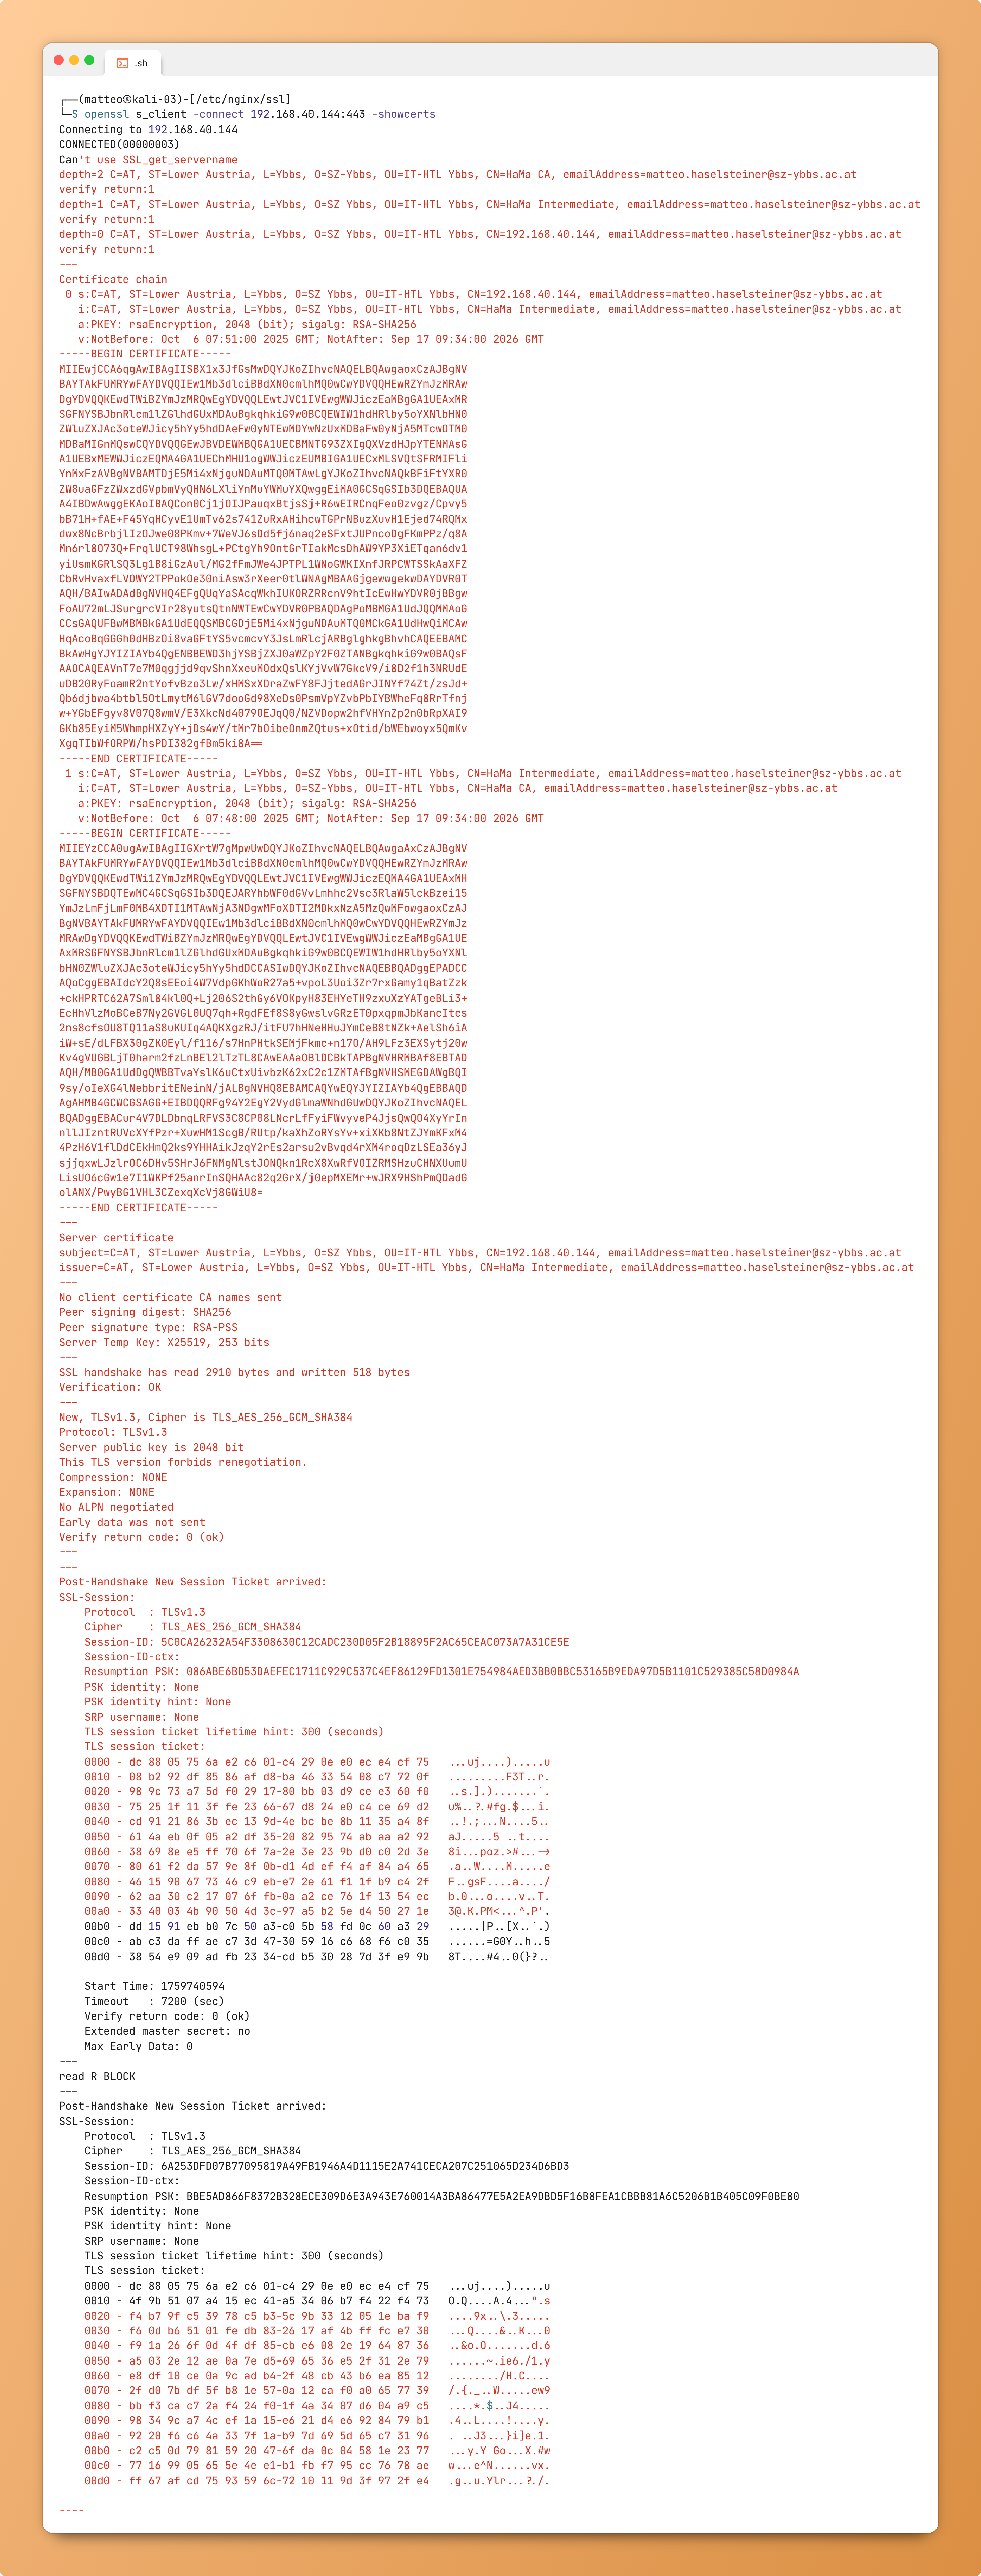
\includegraphics[width=0.8\linewidth]{23-openssl-command.png}
%    \caption{Check Fullchain}
%    \label{fig:screenshot23}
%\end{figure}




%etc.

%% insert bibliography, adds chapter heading with chapter number
% \printbibliography


% \minisec{Zitierbeispiele entsprechend DIN ISO 690}

% Die DIN~ISO~690~\cite{DIN-ISO-690:2013} gibt Hinweise zur vollständigen Quellenangabe.
% Das folgende Beispiele ist dieser Norm entlehnt und angepasst:
% %
% \begin{quotation}
%   Einige Standardwerke \cite{Kohm:20,Voss:22} geben einen guten Überblick über \LaTeX{}.
%   \textcite{Kohm:20} hat die Klassen der KOMA-Script-Reihe entwickelt, die die \enquote{typografischen Gepflogenheiten eines europäischen Layouts berücksichtigen}~\cite[S.~64]{Voss:22}.
%   Daneben empfehlen wir -- nona -- unser Buch zu \LaTeX{}, Excel und Word: \textcite{Schranz:22}.
% \end{quotation}

% Nun der selbe Text in Harvard Citation Style (jedoch ohne \LaTeX-Befehle -- diese wären die selben wie zuvor, es müsste nur der Zitierstil geändert werden):
% %
% \begin{quotation}
%   Einige Standardwerke (Kohm 2020, Voss 2022) geben einen guten Überblick über \LaTeX{}.
%   Kohm (2020) hat die Klassen der KOMA-Script-Reihe entwickelt, die die \enquote{typografischen Gepflogenheiten eines europäischen Layouts berücksichtigen}~(Voss 2022, S.~64).
%   Daneben empfehlen wir -- nona -- unser Buch zu \LaTeX{}, Excel und Word: Schranz et al. (2022).
% \end{quotation}


\end{document}
